\documentclass[a4paper,11pt]{report}

% Packages for document formatting
\usepackage[utf8]{inputenc} % UTF-8 encoding
\usepackage[T1]{fontenc}   % Font encoding
\usepackage{lmodern}       % Improved fonts
\usepackage[a4paper,margin=1.4in]{geometry}      % Page layout
\usepackage{setspace}      % Line spacing
\setstretch{1.2}
\usepackage{titlesec}      % Customizable section titles
\titleformat{\chapter}[display]
  {\normalfont\huge\bfseries}{\chaptername\ \thechapter}{20pt}{\Huge}

% Math and algorithms
\usepackage{amsmath,amssymb,amsfonts} % Math symbols and fonts
\usepackage{amsthm}          % Theorem environments
\usepackage{mathtools}      % Additional math tools
\usepackage{algorithm}
\usepackage{algpseudocode}

% Bibliography management
% \usepackage[backend=biber,style=authoryear]{biblatex} % APA style, customizable
% \addbibresource{ref.bib} % Bibliography file
\usepackage[authoryear]{natbib}  % For author-year citations

% Hyperlinks
\usepackage{hyperref}
\usepackage{cleveref}
\hypersetup{
    colorlinks=true,
    linkcolor=black,
    citecolor=teal,
    filecolor=magenta,
    urlcolor=cyan
    }
\usepackage{cleveref} % Smart referencing

% Acronyms
\usepackage[acronym,nonumberlist]{glossaries}
\makeglossaries
    
% Graphics and tables
\usepackage{graphicx}       % Include images
\usepackage{float}          % Improved figure placement
\usepackage{caption}        % Customizable captions
\usepackage{subcaption}     % Subfigures
\usepackage{booktabs}       % Improved tables
\usepackage{longtable}      % Tables spanning multiple pages


\setlength{\marginparwidth}{2cm}
\usepackage{todonotes}


\theoremstyle{definition}
\newtheorem{definition}{Definition}[section]

\theoremstyle{plain}
\newtheorem{theorem}{Theorem}[section]

\theoremstyle{remark}  % Italicized title, upright text
\newtheorem{remark}{Remark}[section]

\newtheorem{lemma}[theorem]{Lemma}
\newtheorem{corollary}[theorem]{Corollary}
\newtheorem{proposition}[theorem]{Proposition}

\newtheorem{example}{Example}[section]


% Code formatting
\usepackage{listings}       % Include code
\usepackage{xcolor}         % Colors for listings
\lstset{
    basicstyle=\ttfamily\small,
    keywordstyle=\color{blue},
    commentstyle=\color{gray},
    stringstyle=\color{red},
    numbers=left,
    numberstyle=\tiny\color{gray},
    breaklines=true,
    frame=single
}

% Do not edit
% Set up the transparent full-page background logo
\newcommand\BackgroundPicFront{
    \put(-4,0){
        \parbox[b][\paperheight]{\paperwidth}{
            \vfill
            \centering
            {\transparent{0.0}
\includegraphics[width=\paperwidth,height=\paperheight,keepaspectratio]{images/units_logo.png}}
            \vfill
        }
    }
}
% Provides the \thetitle and other useful macros
\usepackage{titling}
\usepackage{tabularx}

% Needed for the transparent full-page background logo
\usepackage{eso-pic}
\usepackage{transparent}

% Thesis's title and author
\title{Reinforcement Learning applications to Minimally invasive Robotic Surgery}
\author{Name Surname}



\begin{document}
\setlength{\parindent}{0pt}

\begin{titlepage}
    \begin{center}
    % Insert the background here
    \AddToShipoutPicture{\BackgroundPicFront}
    {\LARGE {\bfseries UNIVERSITY OF TRIESTE \\}}
    \vspace{5mm}
    {\Large {\bfseries Department of Mathematics, Informatics and Geoscience \\}}
    \vspace{1cm}
    
\includegraphics[width=6cm,height=6cm]{images/units_logo.png}\\[1cm]

    {\LARGE
        Master's Degree in\\ Data Science \& Scientific Computing \\
    }
    \vspace{1cm}
    {\LARGE 
        {\bfseries \thetitle} %
    }
    \todo{trova titolo decente}
    \vspace{1cm}

    % Replace the date with the correct one before printing the final version!
    {\large \today \\[1cm]
    }

    % Table for author's and (co-)supervisor's names
        {\large
            \setlength{\tabcolsep}{12pt}
            \begin{tabularx}{\linewidth}{ >{\raggedleft}X >{\raggedright\arraybackslash}X}
                Candidate & Supervisor \\
                \bfseries Matteo Nunziante & \bfseries Prof. Antonio Celani \\ [2cm] 
                % & Co-supervisor \\
                % & \bfseries Title Name Surname \\ [1cm]
            \end{tabularx}
        }
    A.Y. 2023/2024
    \end{center}
\end{titlepage}


\pagenumbering{roman} % Start with Roman numerals
% Abstract
\chapter*{Abstract}
\addcontentsline{toc}{chapter}{Abstract}
Lung cancer remains a leading cause of cancer-related deaths worldwide, with surgical
resection offering the best chance for cure in early-stage cases. However, the 
intraoperative environment presents significant challenges, including dynamic 
anatomical changes, limited visibility, and high stakes for patient safety. Assistive 
technologies capable of real-time decision-making and adaptability could greatly 
enhance surgical outcomes. In this context, this thesis explores the potential of 
Partially Observable Markov Decision Processes and Reinforcement Learning 
as frameworks for developing intelligent, adaptive, and safe intraoperative AI driven 
systems to support surgeons in Robotic Assisted Surgery.


\chapter*{Thesis Outline and Summary}

There are two major areas that contribute to the advancement of automating surgical procedures: 
perception and task automation. Perception aims at understanding the surgical situation based on 
a variety of inputs during the surgery (endoscopic cameras, tactile feedback etc). This may also include 
the detection, and tracking of surgical tools, as well as 3D reconstruction of the deformed tissue. 
Task automation, on the other hand, involves automating the surgical robot to accomplish specific tasks, 
given the knowledge of the surgical situation. 

Our work focuses on brigding the gap between these two areas, by developing a framework that 
integrates perception and task automation in a single pipeline through the use of Partially Observable 
Markov Decision Processes (POMDPs) and Reinforcement Learning (RL).

% Table of Contents
\tableofcontents
\clearpage
\addcontentsline{toc}{chapter}{List of Figures} % Add to TOC
\listoffigures

\clearpage
\addcontentsline{toc}{chapter}{List of Tables} % Add to TOC
\listoftables

% Acronyms
\addcontentsline{toc}{chapter}{Acronyms}
\newacronym{rl}{RL}{Reinforcement Learning}
\newacronym{dl}{DL}{Deep Learning}
\newacronym{mdp}{MDP}{Markov Decision Process}
\newacronym{pomdp}{POMDP}{Partially Observable Markov Decision Process}
\newacronym{ai}{AI}{Artificial intelligence}
\newacronym{vats}{VATS}{video-assisted thoracic surgery}
\newacronym{rats}{RATS}{robotic-assisted thoracic surgery}
\newacronym{drl}{DRL}{Deep Reinforcement Learning}
\newacronym{gpi}{GPI}{Generalized Policy Iteration}
\newacronym{pbvi}{PBVI}{Point Based Value Iteration}
\newacronym{mc}{MC}{Monte Carlo}
\newacronym{dp}{DP}{Dynamic Programming}
\newacronym{td}{TD}{Temporal Difference}
\printglossary[type=\acronymtype]
\clearpage
\pagenumbering{arabic} % switch to arabic numerals
% Chapters
\chapter{Introduction}

\gls{ai} applications in robotic surgery represent a transformative frontier in the medical field, 
enhancing precision, safety, and efficiency in surgical procedures. 
The integration of such technologies with robotic systems has significantly advanced minimally 
invasive surgery, allowing for smaller incisions, reduced blood loss, and faster recovery times, 
while enabling complex procedures that require exceptional dexterity and visualization capabilities.

Notable robotic systems, such as the da Vinci Surgical System, exemplify the evolution of surgical 
practice through this innovative marriage of AI and robotics, paving the way for improved 
patient outcomes across various specialties, including urology, gynecology, and cardiothoracic surgery.

AI enhances several aspects of surgical practice, including preoperative planning, 
real-time decision support, and postoperative analysis, thereby transforming the surgical landscape.

These advancements underscore AI's potential to refine surgical techniques and foster a culture 
of continuous improvement in surgical care. As the field progresses, the future of AI in robotic 
surgery promises further innovations, such as remote surgical capabilities and enhanced imaging 
technologies, which could redefine healthcare access and delivery on a global scale.



The intersection of AI and robotic surgery not only marks a significant evolution in surgical practices but also holds the potential to fundamentally reshape patient care and outcomes in the coming years.
\gls{rl} in thoracic microinvasive surgery represents a pioneering intersection of artificial intelligence 
and surgical practice, aiming to enhance surgical precision and decision-making processes. 
As robotic-assisted surgical techniques gain traction, particularly through methods like 
\gls{vats} and \gls{rats}, 
the integration of RL algorithms into these workflows has become notable for its potential to 
transform patient outcomes. This application is increasingly relevant as the demand for minimally 
invasive approaches grows, driven by their associated benefits such as reduced postoperative pain 
and shorter recovery times.

The development of \gls{rl} techniques in this field leverages the ability of these algorithms to learn 
from complex interactions within dynamic surgical environments. By training robotic systems to 
optimize intricate tasks through feedback mechanisms, RL not only enhances the operational efficiency 
of surgical robots but also contributes to more informed preoperative planning through predictive 
analytics. 
These advancements allow for tailored risk assessments that improve decision-making in patient care.


Despite its promise, integration of such techniques into thoracic microinvasive surgery faces 
challenges, including the need for robust regulatory frameworks and ongoing ethical scrutiny. 
Discussions surrounding the implications of AI in surgical contexts emphasize the importance of 
ensuring that healthcare providers remain central in the decision-making process while leveraging AI 
technologies to enhance patient care.

Overall, the ongoing research and development in reinforcement learning for thoracic microinvasive 
surgery exemplify a transformative potential in the healthcare landscape, with opportunities for 
improving surgical techniques, outcomes, and training methods while navigating the complexities 
of integrating AI into human-centered care.

% Methodology
\section{Problem Statement}
Over the last decade, 3D models have entered oncologic surgery
as a means to achieve better outcomes in renal and hepatic
surgery [1, 2]. Nevertheless, the integration of 3D models into
the operative field has been lacking due to three main reasons.
Firstly, proper model alignment with the intraoperative anatomy
has proven to be a major challenge due to shifting of organs
during surgery and different patient positioning in surgery ver-
sus during computed tomography [2, 3]. Secondly, automated
organ registra-tion in a continuously moving surgical video
has been another major challenge for many years [4]. Thirdly,
3D model overlay obscures the surgical field, including sharp
surgical instruments which are manipulated, hence creating a
possible hazardous situation rather than facilitating surgery. The
latter occlusion problem has been a longstanding study topic
[5] which, if solved, would further advance various surgical
domains and applications [6]. Already in 2004, Fischer et al. [7]

\paragraph{Navigation in deformable environments}
% Related Work
\section{Related Work}
% Deformable registration refers to the process of aligning multiple three-dimensional 
% images into a common coordinate frame. It quantifies changes in organ shape, size,
% and position, providing a comprehensive understanding of patient anatomy and 
% function. This technique is particularly useful in image-guided surgery and 
% radiotherapy to improve the accuracy of treatments.
\begin{itemize}
    \item Instrument occlusion
    \item DL recognition of anatomical structures
    \item Elastic Regristration
    \item RL for simple surgical tasks
\end{itemize}

While robotic systems have revolutionized minimally invasive surgery, they lack the 
ability to adapt to unexpected intraoperative changes autonomously. \gls{pomdp}s, with 
their capacity to model uncertainty, and RL, with its learning-based adaptability, 
present a promising synergy for addressing these challenges. However, their 
application to real-time intraoperative decision-making remains unexplored.


\paragraph{RL in Surgical Robotics}
\textbf{preso da} \citet{10578312}
ALarge number of recent research in surgical robotics
focuses on the automation of surgical sub-tasks, such
as needle manipulation [1], [2], [3], suturing [4], [5], cutting
[6], [7], [8], vessel manipulation [9], tissue retraction and
deformation [10], [11], [12], [13]. However, most of these
studies focus on the manipulation of rigid and soft objects,
although fluid-related tasks are also common in surgeries, due
to the presence of body fluids, especially blood 


\part{Theoretical Background}


\chapter{Reinforcement Learning}
\todo{controlla itemize}
\begin{itemize}
    \item Bellman Operator is a contraction proof
    \item Q learning convergence experience replay even though convergence
    \item Transfer R Learning ??
    \item 18 Reinforcement Learning in Robotics: A Survey Jens Kober, Jan Peters
    \item Chapter 4
            Learning and Using Models
            Todd Hester and Peter Stone
    \item (P-complete vs. PSPACE-complete)
    \item Gradient and semigradient chap 9 sutton and barto
\end{itemize}

\gls{rl} is a subfield of machine learning focused on the problem of learning 
optimal behaviors: agents repeatedly interact with the environment, balancing 
exploration (trying new strategies) and exploitation (using known strategies) 
to maximize success rate through constant feedback. \

For instance, consider a baby learning to walk: it repeatedly attempts to stand 
and take steps, getting positive feedback for each successful movement and 
negative feedback from falls. Over time, it refines its attempts to walk 
more effectively. \

Differently from supervised learning, where the agent is trained on labeled data, 
and from unsupervised learning, where the agent must find patterns in unlabeled data,
\gls{rl} makes use of rewards and punishments, making it suitable for problems 
where the agent (be it a baby or a Large Language Model) must learn through trial and error, creating its own training data 
through interaction.

% quclosa circa policy e value 
% The concepts of value and value function are key to most of the reinforcement learning
% methods that we consider in this book. We take the position that value functions
% are important for efficient search in the space of policies. The use of value functions
% distinguishes reinforcement learning methods from evolutionary methods that search
% directly in policy space guided by evaluations of entire policies.

% related formal example 
% 
% 
% 
% 

% online vs offline learning
% 
% 
% 
% 
% 

In the next sections, we will introduce the foundational concepts of \gls{rl}, 
mathematical frameworks, and algorithms that enable agents to learn optimal behaviors for 
a wide range of tasks.

The following analysis of \glspl{mdp} is mostly based on \citet{d1afac99aad548188c9d47063c7109df} and \citep{Sutton1998}


\chapter{Markov Decision Processes}

\gls{rl} leverages \glspl{mdp} to model interactions between 
an agent and its environment in terms of states, actions, and rewards. 
This framework captures in a simple way features of the problem such as cause-and-effect, 
uncertainty, and explicit objectives.
Although general \glspl{mdp} may have infinite, possibly uncountable, state and action
spaces, we limit the discussion to finite-state and finite-action problems.

A \gls{mdp} is a model for sequential decision making in a probabilistic environment, it requires
the following components:

\paragraph{States}
The set of environmental states $S$ is defined as the finite set $\{s_1 , . . . , s_N \}$ where the
size of the state space is $|S| = N$. A state is a unique characterization of all
that is important (at given time) of the problem that is modelled. For example, a chess game state 
could be the position of all the pieces on the board.

\paragraph{Actions}
The set of actions A is defined as the finite set $\{a_1 , . . . , a_K \}$ where the size of the
action space is $|A| = K$. Actions can be used to control the system state.
The set of actions that can be applied in some particular state $s \in S$, is denoted $A(s)$,
where $A(s) \subset A$. In some systems, not all actions can be applied in every state, but in
general we will assume that $A(s) = A$ for all $s \in S$.

\paragraph{Trasition Function}
By applying action $a \in A$ in a state $s \in S$, the system makes a transition from s to a
new state $s' \in S$, based on a probability distribution over the set of possible transitions. 
The transition function T is defined as 
$$\mathcal{T} : S \times A \times S \rightarrow [0,1]$$ which represents the probability
of ending up in state s' after doing action a in state s is denoted $ T(s,a,s')$. It is required that 
for all actions a, and all states s and s', $T (s,a,s') \geq 0$ and for all states s and actions a, 
$$\sum_{s' \in S} \mathcal{T} (s,a,s') = 1$$
such that T defines a proper probability distribution over possible next states. \

The sequential nature of the framework is captured by that of \textit{Markov chain}:
a Markovian Stochastic Process. 
Stochastic Processes araise in many problems from the natural sciences
in which one has to keep track of a value observed at time t. The process is Markovian if the result of an action does not
depend on the previous actions and history of visited states, but only depends on the
current state.

Going back to our notation, given a trajectory of the form 
$$s_0, a_0, . . . . , s_t, a_t, s_{t+1}$$
the Markov property is defined as follows:

$$P(s_{t+1} | s_t ,a_t ,s_{t_1} ,a_{t-1} , . . ,s_0,a_0) = P(s_{t+1} | s_t ,a_t ) = \mathcal{T} (s_t ,a_t ,s_{t+1} )$$

The idea of Markovian dynamics is that the current state s gives enough information
to make an optimal decision; it is not important which states and actions preceded s.

\paragraph{Reward Function}
Rewards guide learning by signaling success. A higher reward indicates a more 
desirable outcome. In the chess example, capturing a piece might give a large reward, encouraging the 
agent to repeat the actions that led to that success. The reward function R is usually defined as
$$R : S \times A \times S \rightarrow [0,1]$$
which represents the reward received after transitioning from state $s$ to $s'$ by taking action $a$.
Alternatively, the reward function can be defined as $R : S \times A \rightarrow \mathbb{R}$, 
where the reward depends only on the current state and action. \\


\ With the above components, we can define a \gls{mdp} as in \Cref{fig:mdp}.

\begin{definition}
A \textit{Markov Decision Process} is a tuple $M = (S, A, \mathcal{T}, \mathcal{R})$ where:
\begin{itemize}
    \setlength\itemsep{0.01em}
    \item $S$ is a finite set of states
    \item $A$ is a finite set of actions
    \item $\mathcal{T}$ is the transition function $\mathcal{T} : S \times A \times S \rightarrow [0,1]$
    \item $\mathcal{R}$ is the reward function $\mathcal{R} : S \times A \times S \rightarrow \mathbb{R}$
\end{itemize}
\end{definition}
The transition and reward functions together define the \textbf{Model} of
the \gls{mdp}.

\begin{figure}[H]
    \centering
    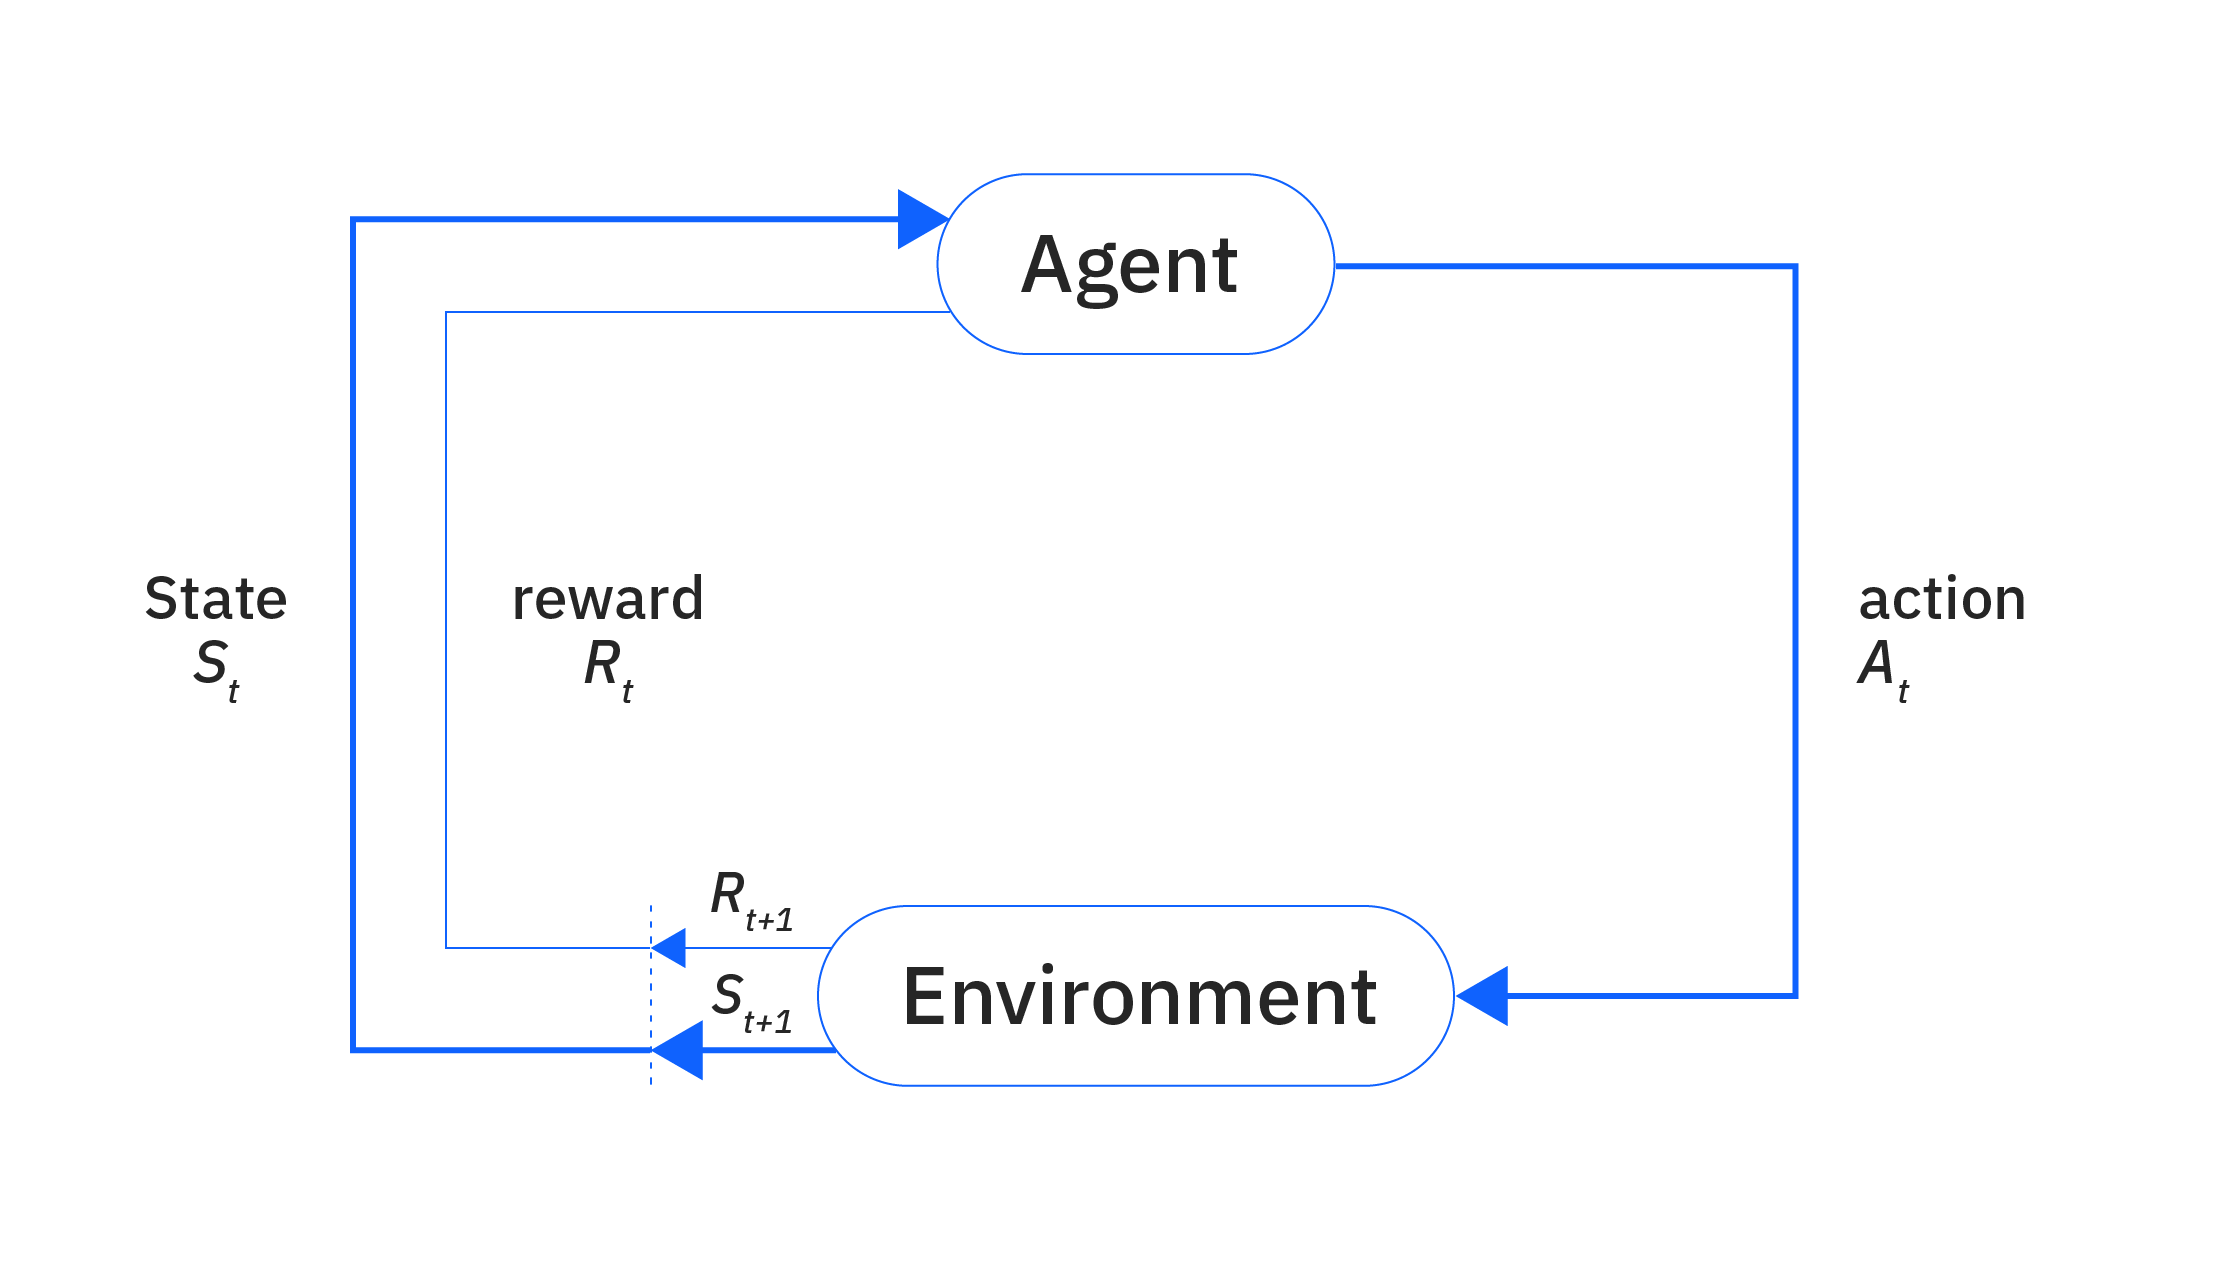
\includegraphics[width=0.5\textwidth]{images/MDP.png}
    \caption{Markov Decision Process}
    \label{fig:mdp}
\end{figure}

A unified notion of Transitions and Rewards is given by what's called the dynamic of the \gls{mdp}
$$p : S \times R \times S \times A \rightarrow [0, 1]$$
where
$$p(s' , r |s, a) = Pr\{S_t = s' , R_t = r | S_{t-1} = s, A_{t-1}= a\}$$

$p$ is an ordinary deterministic function of four arguments and the ‘|’ in the middle of it 
comes from the notation for conditional probability, note that the following holds:
$$\sum_{s^{\prime} \in S} \sum_{r \in R} p\left(s^{\prime}, r \mid s, a\right)=1 \text {, for all } s \in S, a \in A(s) \text {. }  $$
    
$$
p\left(s^{\prime} \mid s, a\right) \doteq \operatorname{Pr}\left\{S_{t}=s^{\prime} \mid S_{t-1}=s, A_{t-1}=a\right\}=\sum_{r \in R} p\left(s^{\prime}, r \mid s, a\right).
$$
as for \(r: S \times A \times S \rightarrow \mathbb{R}\),
$$
r\left(s, a, s^{\prime}\right) \doteq \mathbb{E}\left[R_{t} \mid S_{t-1}=s, A_{t-1}=a, S_{t}=s^{\prime}\right]=\sum_{r \in \mathcal{R}} r \frac{p\left(s^{\prime}, r \mid s, a\right)}{p\left(s^{\prime} \mid s, a\right)}
$$

these formulations are useful for the analysis of the \gls{mdp} and the development of algorithms. 
In such context, the goal of the agent is to learn an optimal behaviour. 
Thus, let's define behaviours and optimality.

\section{Policy and Value Function}
\paragraph{Policy}
The formalization of the naive concept of behaviour is that of policy. A policy is a function that 
maps states into actions $\pi : S \rightarrow A$. It can be deterministic or stochastic, in 
the latter case it is represented as a probability distribution over actions given states.

$$\pi(a|s) = Pr\{A_t = a | S_t = s\}$$

it holds that for all states $s \in S$, $\pi(a|s) \geq 0$ and $\sum_{a \in A} \pi(a|s) = 1$. \
Such policy represents the strategy of the agent, it is the way the agent interacts with the environment
by iteratively selecting actions based on the current state of the system and thereby influencing the next state and 
reward received. \\
The main goal of \gls{rl} is to find "good" policies. It is intuitive to think that a policy is good 
if it produces high rewards.

\todo{add nonstationary definition of policy}
% We consider two kinds of policies:
% stationary and nonstationary. A stationary policy, n : S -+ A,is a situation-action mapping
% that specifies, for each state, an action to be taken. The choice of action depends only on the
% state and is independent of the time step. A nonstationary policy is a sequence of situation-
% action mappings, indexed by time. The policy rrt is to be used to choose the action on the
% tth-to-last step as a function of the current state, St. In the finite-horizon model, the optimal
% policy is not typically stationary: the way an agent chooses its actions on the last step of its
% life is generally going to be very different from the way it chooses them when it has a long
% life ahead of it. In the infinite-horizon discounted model, the agent always has a constant
% expected amount of time remaining, so there is no reason to change action strategies: there
% is a stationary optimal policy.   

\paragraph{Value Function} The concept of value function is useful to evaluate the 
quality of a policy. The value function of a state \(s\) under a policy \(\pi\), denoted \(V^{\pi}(s)\), 
is the expected return when starting in \(s\) and following \(\pi\) thereafter. 
We can define the state-value function  \(V^{\pi}\)  for policy \(\pi\) by

$$
V^{\pi}(s) \doteq 
\mathbb{E}_{\pi}\left[\sum_{k=0}^{\infty} \gamma^{k} R_{t+k+1} \mid S_{t}=s \right]
 \text {, for all } s \in S, \quad
$$
% \mathbb{E}_{\pi}\left[G_{t} \mid S_{t}=s\right] 

where \(\mathbb{E}_{\pi}[\cdot]\) denotes the expected value of a random variable given that the agent follows
policy \(\pi\), and \(t\) is any time step, $\gamma \in [0,1]$ is the discount factor, it is used 
to weigh the importance of immediate rewards and to make sure that the sum converges even in 
infinite horizon problems.

\begin{align}   
V^{\pi}(s)&=E{\left[\sum_{k} \gamma^k R_{t+k+1}+|S_t=s\right]} \nonumber \\
&=E{\left[G_t|S_t=s\right]} \nonumber \\
&=E{\left[R_{t+1}+\gamma G_{t+1}|S_t=s\right]} \nonumber \\
&= \sum_{s'}\sum_{r}\sum_{g_{t+1}}\sum_{a}p(s',r,g_{t+1}, a|s)(r+\gamma g_{t+1}) \nonumber \\
&= \sum_{a}\pi(a|s)\sum_{s'}\sum_{r}\sum_{g_{t+1}}p(s',r,g_{t+1} |a, s)(r+\gamma g_{t+1}) \nonumber \\
\intertext{since $p(g_{t+1}|s', r, a, s)=p(g_{t+1}|s')$ by MDP assumption}
&= \sum_{a}\pi(a|s)\sum_{s'}\sum_{r}\sum_{g_{t+1}}p(s',r|a, s)p(g_{t+1}|s', r, a, s)(r+\gamma g_{t+1}) \nonumber \\
&= \sum_{a}\pi(a|s)\sum_{s'}\sum_{r}p(s',r|a, s)\sum_{g_{t+1}}p(g_{t+1}|s')(r+\gamma g_{t+1}) \nonumber \\
&= \sum_{a}\pi(a|s)\sum_{s'}\sum_{r}p(s',r|a, s)(r+\gamma\sum_{g_{t+1}}p(g_{t+1}|s')g_{t+1}) \nonumber \\
&=\sum_{a}\pi(a|s)\sum_{s'}\sum_{r}p(s',r|a, s)\left(r+\gamma V^{\pi}(s')\right) \label{eq2}
\end{align}
% notice that p(s',r|s,a) = p(s',r,a|s)p(a|s) allora l'expected value è sum su a s'

Eq \ref{eq2} is a famous recoursive relationship know as the \textit{Bellman equation} for 
$V^{\pi}$, forming the basis to learn, compute and approximate the value function.


Similarly one can define the state-action value function, giving value of taking action \(a\) in 
state \(s\) under a policy \(\pi\), denoted
$Q^{\pi}(s, a): S \times A \rightarrow \mathbb{R}$, as the expected return starting from \(s\), taking the action \(a\), and thereafter
 following policy \(\pi\) :
\begin{align}
    Q^{\pi}(s, a) &\doteq \mathbb{E}_{\pi}\left[\sum_{k=0}^{\infty} \gamma^{k} R_{t+k+1} | S_{t}=s, A_{t}=a\right] \nonumber  \\
    &= \mathbb{E}_{\pi}\left[R_t + \gamma V^{\pi}(S_{t+1})| S_{t}=s, A_{t}=a\right] 
\end{align}


it follows naturally that 
\[
    V^{\pi}(s)= \max _{a \in A(s)} Q^{\pi}(s, a)
\]

\section{Bellman Optimality Equation}

Introducing a partial ordering on the space of policies such that 

$\pi \geq \pi' \text{ if and only if } V^{\pi}(s) \geq V^{\pi'}(s) \text{ for all } s \in S$
allows to compare different policies, and to define optimal ones as the class $\pi^*$ 
$$\pi^* \text{ such that } \pi^* \geq \pi \text{ for all } \pi$$

% l'ordine è parziale perchè non è detto che >= valga per ogni s in S ma potrebbe valere solo per alcuni a quel punto non sono confrontabili

\glspl{mdp} (but not \glspl{pomdp}, we'll introduce them in the next chapter), there always\footnote{This 
is true in discrete state space \gls{mdp}s when $\gamma < 1$. 
Existence of optimal policies is not guaranteed in discrete problems for $\gamma = 1$. Generally 
it is required $\gamma \in (0,1)$, and costs (negative rewards) to be bounded $|c(s,a)|<M$ for all s and a in a continous setting}
 is a 
deterministic, stationary (time independent) policy that maximizes the value of every state. \cite{96ef8573-56cc-3a43-a4c7-3c6543c30f4e}
% qualcuno vuole dimostrare l'esistenda stazionarietà e determinismo dell'optimal policy in MDP
    
If we know this optimal policy, then we get the optimal value function $V^{*}(s_{t})$:
\[
V^{*}(s)=\max _{\pi}V^{\pi}(s)
\]
 Similarly, the optimal state-action value function is obtained under the optimal policy:
$$
Q^{*}\left[s_{t}, a_{t}\right]=\max _{\pi} Q^{\pi}\left(s_{t}, a_{t}\right)
$$

Vice versa, knowing the optimal state-action value function allows to derive the optimal policy by 
choosing the action \(a_{t}\) with the highest value
\[
\pi^*\left(s_{t}\right) = \underset{a_{t}}{\operatorname{argmax}}\left[Q^{*}\left(s_{t}, a_{t}\right)\right]
\]

The optimal value function satisfies the \textit{Bellman Optimality Equation}, given by:

\begin{align}
    V^{\ast }(s)&=\max\limits_{a\in A(s)}Q^{\pi _{\ast }}(s,a) \nonumber \\ 
    & =\max\limits_{a}\mathbb{E}_{\pi _{\ast }}[G_{t}\mid S_{t}=s,A_{t}=a] \nonumber \\ 
    & =\max\limits_{a}\mathbb{E}_{\pi _{\ast }}[R_{t+1}+\gamma G_{t+1}\mid
    S_{t}=s,A_{t}=a] \nonumber \\ 
    & =\max\limits_{a}\mathbb{E}[R_{t+1}+\gamma V^{\ast }(S_{t+1})\mid
    S_{t}=s,A_{t}=a] \nonumber \\ 
    & =\max\limits_{a}\sum\limits_{s^{\prime },r}p(s^{\prime
    },r\mid s,a)\left[ r+\gamma V^{\ast }(s^{\prime })\right].%
    \label{Bellman-optimality-eq}
\end{align}

An analogous result holds for the optimal state-action value function:
\begin{align}
    Q^{\ast }(s,a)&=\mathbb{E}[R_{t+1}+\gamma\max\limits_{a^{\prime }}Q^{\ast
    }(S_{t+1},A_{t+1})\mid S_{t}=s,A_{t}=a] \nonumber \\ 
    & =\sum\limits_{s^{\prime },r}p(s^{\prime },r\mid s,a)\left[ r+\gamma\max\limits_{a^{\prime }}Q^{\ast }(s^{\prime },a^{\prime })\right]. \\
    & = \sum_{s^{\prime}, r} p(s^{\prime}, r | s, a) \left[ r + \gamma V^*(s') \right]
    \label{eq:bellman-state-action}
\end{align}


These equations must be satisfied and can, in principle, be solved for the optimal
value functions, from which an optimal policy can be determined with relative ease.
In practice this is hardly the case due to computational limitations and the optimal value functions 
are usually approximated.

\section{Solving MDPs}
Solving a given \gls{mdp} means computing an optimal policy. The most crucial distinction in available techniques 
is that between model-based and model-free algorithms. 
Model-based methods use the \gls{mdp} structure explicitly and find the best policy from the transition and reward functions.
If these are known, this is a straightforward optimization problem that can be tackled using dynamic programming. 
If they are unknown, they must first be estimated from observed trajectories.
{\todo{da spinningup}
The main upside to having a model is that it allows the agent to plan by thinking ahead, 
seeing what would happen for a range of possible choices, and explicitly deciding between its options. 
Agents can then distill the results from planning ahead into a learned policy. 
A particularly famous example of this approach is AlphaZero.\cite{Silver2017} 
When this works, it can result in a substantial improvement in sample efficiency over methods that don't 
have a model. \cite{SpinningUp2018}

The main downside is that a ground-truth model of the environment is usually not available to the agent. 
If an agent wants to use a model in this case, it has to learn the model purely from experience, which 
creates several challenges.
}
Modern solution methods - entirely based on \gls{drl} - presented in fig. \ref{fig:drl-algorithm-evolution}, rely on 
Neural Networks to approximate the value function, the policy, or both. \\

Before diving into these methods, we will introduce some of the most common and foundational algorithms 
used to solve \glspl{mdp} that are the building blocks of more advanced techniques.

\begin{figure}
    \centering
    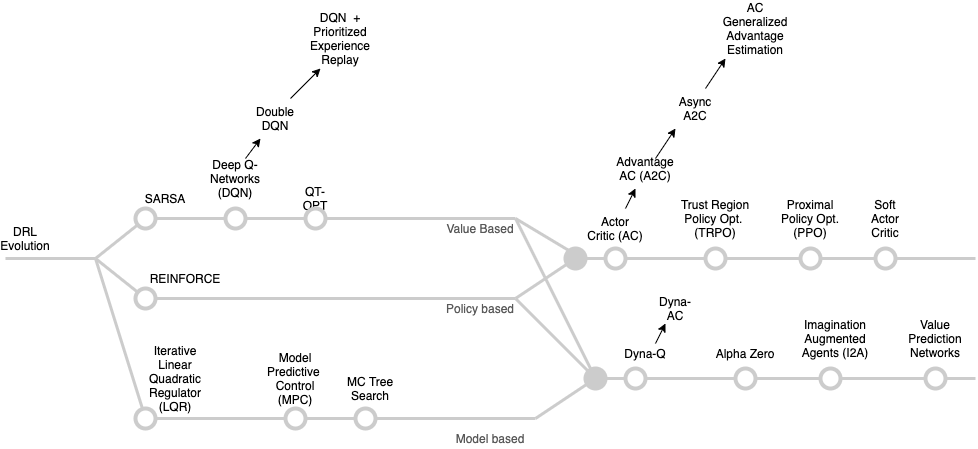
\includegraphics[scale=.35]{images/drl-algorithm-evolution.png}
    \caption{Evolution of Deep Reinforcement Learning Algorithms}
    \label{fig:drl-algorithm-evolution}
\end{figure}

\section{Dynamic Programming}
Dynamic Programming (DP) is a class of algoritms of little practical use, nontheless of great theoretical 
importance in the field of model-based \gls{rl}. The assumption of the availability of the model is 
crucial for the application of these methods as the finitenees of the state and action spaces, though 
continous spaces can be discretized, exact solutions can be rarely found. 
Two main steps are involved: policy evaluation and policy improvement.

\paragraph{Policy Evaluation} Recall that policy evaluation or prediction is the task of determining 
the value function of a given policy. If the environment's dynamics are known, \Cref{eq2} represents 
a linear system in the $|S|$ unknowns $V^{\pi}(s)$, which can be solved exactly or iteratively. Due 
to the computational burden of exact solutions, iterative methods are preferred. The most famous of these 
known as \textit{Iterative Policy Evaluation} is based on the \textit{Bellman Equation}:

$$V^{k+1}(s) = \sum_{a}\pi(a|s)\sum_{s'}\sum_{r}p(s',r|a, s)(r+\gamma V^{k}(s'))$$

where $V^{k}(s)$ is the value function at iteration $k$. The algorithm is guaranteed to converge to the 
true value function $V^{\pi}$ as $k \rightarrow \infty$ under the assumption that $\gamma < 1$ as a 
consequence of the contraction property of the Bellman operator. See \Cref{lemma:contraction} for 
a similar argument.

\paragraph{Policy Improvement} 
The purpose of calculating the value function for a policy is to identify better policies. 
To determine if a policy can be improved, we 
compare the value of taking a different action \( a \) in state \( s \) with the current policy. 
This is done using the state-action value function \( Q^\pi(s, a) \) as in equation [manca cit equation]:
If $Q^\pi(s, a) > V^\pi(s)$, choosing action $a$ in $s$ is more advantageous than following $\pi$, 
leading to an improved policy $\pi'$. 
\begin{align}
    \pi'(s) & \doteq arg\max_a Q^\pi(s,a) \nonumber\\
    &=  \mathbb{E}[R_{t+1}+\gamma V^{\pi}(S_{t+1})\mid S_t=s,A_t=a] \nonumber\\
    &= arg\max _a \sum_{s', r} p(s',r\,|s,a)\Big[r+\gamma V^{\pi}(s')\Big] \nonumber\\
    \label{eq:policy-improvement}
\end{align}

This is motivated by the following theorem:
\begin{theorem}
    (Policy Improvement Theorem) Let $\pi$ and $\pi'$ be any pair of deterministic policies such that, 
    for all $s \in S$ 
    $$Q^\pi(s, \pi'(s)) \geq V^\pi(s)$$
    Then the policy $\pi' \geq \pi$. That is, it must obtain greater 
    or equal expected return from all states $s \in S$:
    $$V^{\pi'}(s) \geq V^\pi(s)$$
    If there is strict inequality at any state, $\pi'$ is superior to $\pi$.
    \label{th:policy-improvement}
\end{theorem}
\begin{proof}
    \begin{align}
        V^{\pi}(s) &\leq Q^{\pi}(s, \pi'(s)) \nonumber \\
        &= \mathbb{E}\left[R_{t+1} + \gamma V^{\pi}(S_{t+1}) | S_t = s\right] \nonumber \\
        &\leq \mathbb{E}\left[R_{t+1} +\gamma Q^{\pi}(S_{t+1}, \pi'(S_{t+1})) | S_t = s\right] \nonumber \\
        &= \mathbb{E}\left[R_{t+1} + \gamma R_{t+2} + \gamma ^2 V^{\pi}(S_{t+1}) | S_t = s\right] \nonumber \\
        &\leq \dots \nonumber \\
        &=V^{\pi'}(s) \nonumber
    \end{align}
\end{proof}

% \begin{align}
% \pi'(s) &\equiv \arg\max_a Q^\pi(s, a) \nonumber\\
% &= \arg\max_a \mathbb{E}[\mathcal{R}_{t+1} + \gamma V^\pi(\mathcal{S}_{t+1}) \mid \mathcal{S}_t = s, \mathcal{A}_t = a] \nonumber\\
% &= \arg\max_a \sum_{s', r} p(s', r \mid s, a) [r + \gamma V^\pi(s')]  \nonumber
% \end{align}

Policy improvement creates a new policy that enhances an initial policy by adopting a greedy approach 
based on the value function.

To show convergence to the optimal policy, along with monotone
improvement, we need to show that if there is no improvement in the value function at any state, then we
are at optimality. Consider k such that 
$V^{\pi_{k+1}} (s) = V^{\pi_{k}}(s), \forall s \in S$. 
We can show using \cref{eq:policy-improvement} that such $V^{\pi_{k}}$ satisfies the Bellman Optimality equation 
\ref{Bellman-optimality-eq}, and hence $V^{\pi_{k}} = V^*$.

\subsection{Policy Iteration}
Policy Iteration allows to estimate an optimal policy in finite time. It is the combination of Policy 
Evaluation and Policy Improvement: once a policy $\pi_t$, has been improved using $V_{t-1}$ to yield 
a better policy $\pi_{t+1}$, we can then compute $V_{t+1}$ and start again. 
\[
\quad \pi_0 \stackrel{\rm E}{\longrightarrow} v_{\pi_0} \stackrel{\rm I}{\longrightarrow} \pi_1 \stackrel{\rm E}{\longrightarrow} v_{\pi_1} \stackrel{\rm I}{\longrightarrow} \pi_2 \stackrel{\rm E}{\longrightarrow} \cdots \stackrel{\rm I}{\longrightarrow} \pi_* \stackrel{\rm E}{\longrightarrow} v_*, \quad
\]
By previous results we can thus obtain a sequence of monotonically improving policies and value functions 
unless we reach the optimal policy. Convergence is guaranteed by the finiteness of the \gls{mdp}.
The algorithm is summarized in \ref{alg:policy-iteration}.

\begin{algorithm}[H]
    \caption{Policy Iteration}\label{alg:policy-iteration}
    \begin{algorithmic}
    \Require A finite \gls{mdp} with states $S$, actions $A$, transition probabilities $T$, rewards $R$, and discount factor $\gamma \in [0,1]$
    \Ensure Optimal policy $\pi^*$
    \State Initialize an arbitrary policy $\pi$
    \Repeat
        \State \textbf{Policy Evaluation:} Compute the state-value function $V^\pi$
        \State Solve $V^\pi(s) = \sum_{a \in A} \pi(a|s) \sum_{s' \in S} T(s' | s, a) \left[ R(s, a, s') + \gamma V^\pi(s') \right]$ for all $s \in S$
        \State \textbf{Policy Improvement:} Compute a new policy $\pi'$
        \ForAll{$s \in S$}
            \State $\pi'(s) \gets \arg\max_{a \in A} \sum_{s' \in S} T(s' | s, a) \left[ R(s, a, s') + \gamma V^\pi(s') \right]$
        \EndFor
    \Until{$\pi' = \pi$}  \Comment{Stop when policy converges}
    \State \Return $\pi^*$
    \end{algorithmic}
\end{algorithm}

\subsection{Value Iteration}
The main drawback of Policy Iteration is the need to perform the time comsumnic policy 
evaluation stepat each iteration.
Value Iteration is a simpler alternative that works by truncating the policy evaluation step 
without loosing convergence guarantees. 
Truncating the policy evaluation step after a single sweep, results in the following update rule for the 
value function:
\[
\begin{array}{lll}
V_{k+1}(s) & \doteq & \displaystyle \max_{a} \mathbb{E}[R_{t+1}+\gamma V_k(S_{t+1}) \mid S_t=s, A_t=a] \\ 
& = & \displaystyle \max_{a} \sum\limits_{s',r} p(s',r \mid s, a) \left[r+\gamma V_k(s')\right],
\end{array}
\]

or in the equivalent form $V_{t+1} = BV_t$
where $B$ is the Bellman Optimality Operator defined as: 
\begin{equation}
    (B^*V)(s) = \max_{a} \sum_{s',r} p(s',r|s,a) \left[ r + \gamma V(s') \right]
    \label{eq:bellman-operator}
\end{equation}
The foundamental theoretical result is that the sequence of value functions $\{V_k\}$ converges to the optimal
value function $V^*$ as $k \rightarrow \infty$.

\begin{lemma}
    The Bellman Optimality operator $B^*$ is a contraction mapping with respect to the
    supremum norm.
    \label{lemma:contraction}
\end{lemma}
\begin{proof}
    Let $V, W$ be any two value functions. Then, for all $s \in S$:
    \begin{align*}
        |(B^*V)(s) - (B^*W)(s)| &= \left| \max_{a} \sum_{s',r} p(s',r|s,a) \left[ r + \gamma V(s') \right] - \max_{a} \sum_{s',r} p(s',r|s,a) \left[ r + \gamma W(s') \right] \right| \\
        &\leq \max_{a} \left| \sum_{s',r} p(s',r|s,a) \left[ r + \gamma V(s') \right] - \sum_{s',r} p(s',r|s,a) \left[ r + \gamma W(s') \right] \right| \\
        &\leq \max_{a} \sum_{s',r} p(s',r|s,a) \left| \left[ r + \gamma V(s') \right] - \left[ r + \gamma W(s') \right] \right| \\
        &\leq \max_{a} \sum_{s'} p(s'|s,a) \left| \gamma V(s') - \gamma W(s') \right| \\
        &\leq \gamma \max_{a} \sum_{s'} p(s'|s,a) \left| V(s') - W(s') \right| \\
        &\leq \gamma \max_{a} \left\| V - W \right\|_{\infty}
    \end{align*}
    where $\left\| V - W \right\|_{\infty} = \max_{s \in S} |V(s) - W(s)|$ is the supremum norm.
\end{proof}

\begin{theorem}
    (Value Iteration Convergence) The sequence of value functions $\{V_k\}$ generated by the value iteration 
    algorithm converges to the optimal value function $V^*$ as $k \rightarrow \infty$.
\end{theorem}
\begin{proof}
    The result is direct consequence of the contraction property of the Bellman Optimality operator 
    and the Banach Fixed-Point Theorem.
    \begin{align*}
        \left\| V_{k+1} - V^* \right\|_{\infty} &= \left\| B^*V_k - B^*V^* \right\|_{\infty} \\
        &\leq \gamma \left\| V_k - V^* \right\|_{\infty}
    \end{align*}
    By induction, we have that $\left\| V_k - V^* \right\|_{\infty} \leq \gamma^k \left\| V_0 - V^* \right\|_{\infty}$.
    Since $\gamma \in [0,1)$, the sequence $\{V_k\}$ converges to $V^*$.

\end{proof}
The algorithm is summarized in \ref{alg:value_iteration}.

\begin{algorithm}[H]
    \caption{Value Iteration}\label{alg:value_iteration}
    \begin{algorithmic}
    \Require A finite \gls{mdp} with states $S$, actions $A$, transition probabilities $T$, rewards $R$, discount factor $\gamma \in [0,1]$, and a small threshold $\theta > 0$
    \Ensure Optimal policy $\pi^*$
    \State Initialize value function $V(s) \gets 0$ for all $s \in S$
    \Repeat
        \State $\Delta \gets 0$
        \ForAll{$s \in S$}
            \State $v \gets V(s)$
            \State $V(s) \gets \max_{a \in A} \sum_{s' \in S} P(s' | s, a) \left[ R(s, a, s') + \gamma V(s') \right]$
            \State $\Delta \gets \max(\Delta, |v - V(s)|)$
        \EndFor
    \Until{$\Delta < \theta$}  \Comment{Stop when value function converges}
    \State \textbf{Extract Policy:}
    \ForAll{$s \in S$}
        \State $\pi^*(s) \gets \arg\max_{a \in A} \sum_{s' \in S} P(s' | s, a) \left[ R(s, a, s') + \gamma V(s') \right]$
    \EndFor
    \State \Return $\pi^*$
    \end{algorithmic}
\end{algorithm}

\subsection{Generalized Policy Iteration}
A very important underlying mechanism, common to most methods, is the so-called \gls{gpi} principle. 
It consists of two interacting processes. 

The policy evaluation step estimates the utility
of the current policy, that is, it computes $V^{\pi}$, directly through the use of the model (if available)
or iteratively by sampling trajectories interacting with the environment

The policy improvement step.  
This step computes an improved policy from the current one using the information in $V$. 

Both the evaluation and the improvement steps can be implemented in
various ways, and interleaved in several distinct ways. The bottom line is that there
is a policy that drives value learning, i.e. it determines the value function, but in
turn there is a value function that can be used by the policy to select good actions.

\begin{figure}
    \centering
    \includegraphics[scale=.2]{images/gpi.png}
    \caption{Generalized Policy Iteration}
    \label{fig:gpi}
\end{figure}



\section{Monte Carlo Methods}
Learning methods do not necessarly need to rely on the model of the environment. Model free techniques 
are based on the idea of learning from experience - actual or simulated\footnote{Although a model is 
needed for simulated experience, it can be a sample model which is way easier to obtain than a 
full probabilistic specification of the environment dynamics} - in the form of sample sequence of states, 
actions and rewards.
Following the \gls{gpi} framework we breafly explore the main ideas behind \gls{mc} Methods.

\paragraph{Policy Evaluation} The most simple strtegy for estimating the value function without a model 
is to average rewards after visiting a state.
In particular, if we had to estimate $V_{\pi}(s)$, given a set of episodes obtained by following ${\pi}$
after s, since s may be visited multiple times in the same episode; denoting the first time it is 
visited in an episode the \textit{first visit} to s, two options are available:
\begin{itemize}
    \item First-visit \gls{mc} method estimates V(s) as the average of the returns following first visits to s
    \item Every-visit \gls{mc} method averages the returns following all visits to s.
\end{itemize}

Convergence of both methods is guaranteed by the law of large numbers.

\paragraph{Policy improvement}
It is worth noting that the absence of the model, state values alone are not sufficient to determine a 
greedy policy wrt $V$, \gls{mc} methods are therefore used to estimate the action-value function
$Q_{\pi} (s, a)$ for control tasks. 
The concept of visits is redefined to apply to state-action pairs, rather than states alone. A state-action pair (s, a) is considered visited if action a was selected while in state s

\paragraph{Monte Carlo Control}
While Policy Evaluation and Improvement, we need to be cautious and ensure that all
states will be visited, otherwise convergence is not guaranteed. To accomplish this we can generate the 
episodes with \textit{exploring starts}, that is, all episodes begin with state-action pairs randomly
selected to cover all possibilities.
The second underlying assumption we made is that policy evaluation could be done over an infinite number of 
episodes. Under theses assumptions, the value function converges to the true value function thanks to 
the \textit{Policy Improvement Theorem} \ref{th:policy-improvement}. 

Both assumptions can actually be relaxed by giving up on deterministic policies and only search over
$\epsilon$-soft policies and by using allowing the value function to be updated after each episode and 
not when convergence is met.

$$
\pi(a|s)=\left\{
\begin{array}{ll}
1-\epsilon+\frac{\epsilon}{|A|} & \mbox{if $a=\mbox{argmax}_{a'}Q_{\pi}(s,a')$} \\
\frac{\epsilon}{|A|} & \mbox{otherwise}
\end{array}
\right.
$$


\begin{algorithm}
    \caption{Monte Carlo Control with Exploring Starts}\label{alg:monte_carlo}
    \begin{algorithmic}
    \Require A finite \gls{mdp} with states $S$, actions $A$, rewards $R$, discount factor $\gamma \in [0,1]$, and an exploring-starts assumption
    \Ensure Optimal policy $\pi^*$
    
    \State Initialize arbitrary action-value function $Q(s, a)$ for all $s \in S$, $a \in A$
    \State Initialize returns list $\text{Returns}(s, a) \gets \emptyset$ for all $s, a$
    \State Initialize policy $\pi$ arbitrarily
    \Repeat
        \State Generate an episode: $(s_0, a_0, r_1, s_1, a_1, r_2, \dots, s_T)$ following $\pi$
        \State $G \gets 0$
        \For{$t = T-1$ to $0$}  \Comment{Process the episode in reverse}
            \State $G \gets \gamma G + r_{t+1}$
            \If{$(s_t, a_t)$ is the first occurrence in the episode}
                \State Append $G$ to $\text{Returns}(s_t, a_t)$
                \State $Q(s_t, a_t) \gets \frac{1}{|\text{Returns}(s_t, a_t)|} \sum \text{Returns}(s_t, a_t)$
                \State Update policy: $\pi(s_t) \gets \arg\max_{a \in A} Q(s_t, a)$
            \EndIf
        \EndFor
    \Until{Q-values converge}
    
    \State \Return $\pi^*$
    \end{algorithmic}
\end{algorithm}


\section{Temporal Difference Learning}
Combining the ideas of \gls{dp} and \gls{mc} methods, \gls{td} learning is a model-free method that 
learns from experience (like \gls{mc}) but updates estimates based on other learned estimates 
(like \gls{dp}), a technique known as bootstrapping.

\gls{td} prediction methods update the value function estimates based on the difference between the
current estimate and a target value, which is a sum of the reward and the value of the next state.
The simplest form of \gls{td} learning is the \gls{td}(0) algorithm, also known as the one-step \gls{td}
algorithm. The update rule for the value function is given by:
\[
V(S_t) \leftarrow V(S_t) + \alpha \Big[ R_{t+1} + \gamma V(S_{t+1}) - V(S_t) \Big]
\]
Convergence results for TD(0) is found in \cite{10.1023/A:1022633531479}, For any fixed policy $\pi$, 
TD(0) has
been proved to converge to $V_\pi$, in the mean for a constant step-size parameter if it is
sufficiently small, and with probability 1 if the step-size parameter decreases according to
the usual stochastic approximation conditions
\[
\sum_{n=1}^{\infty}\alpha_{n}(a)=\infty\quad\quad\quad\mbox{and}\quad\quad\sum_{n=1}^{\infty}\alpha_{n}^{2}(a)<\infty.
\]

We present two \gls{td} control methods that are widely used in practice: Sarsa and Q-Learning.

\subsection{Sarsa} Sarsa is an on-policy method that updates the action-value function Q based on the
current policy $\pi$ and the action taken in the next state. The update rule is given by:

\[
Q(S_t,A_t) \leftarrow Q(S_t,A_t) + \alpha \Big[ R_{t+1} + \gamma Q(S_{t+1},a) - Q(S_t,A_t) \Big].
\]

The convergence properties of the Sarsa algorithm depend on the nature of the policy’s
dependence on Q. For example, one could use "-greedy or "-soft policies. Sarsa converges
with probability 1 to an optimal policy and action-value function as long as all state–action
pairs are visited an infinite number of times and the policy converges in the limit to
the greedy policy

\subsection{Q-Learning}
A similar update for an off-policy method is given by the Q-Learning algorithm (Watkins, 1989), 
which update
\[
Q(S_t,A_t) \leftarrow Q(S_t,A_t) + \alpha \Big[ R_{t+1} + \gamma \max_a Q(S_{t+1},a) - Q(S_t,A_t) \Big].
\]
In this case, the learned action-value function, Q, directly approximates q , the optimal
action-value function, independent of the policy being followed. This dramatically
simplifies the analysis of the algorithm and enabled early convergence proofs. The policy
still has a crucial role in that it determines which state-action pairs are visited,
and it is required for convergence that all pairs continue to be updated.

Q-learning is one of the most well known and widely used algorithms in \gls{rl} and has been
extended and adapted in many ways. The convergence of Q-learning has been proved for
many cases, including linear function approximation, and it has been shown to be a very
effective and robust method in practice.

\section{Policy Gradient Methods}


\chapter{Partially Observable Markov Decision Processes}


Until now we have considered the case of fully observable \glspl{mdp}, 
where the agent has access to the complete state of the environment. This is not always the case, 
and in many real-world scenarios, the agent has only partial information about the state of the environment. 
As \glspl{mdp} are controlled Markov Chains, \glspl{pomdp} are controlled Hidden Markov Models \Cref{fig:pomdp}.
\begin{figure}[H]
    \centering
    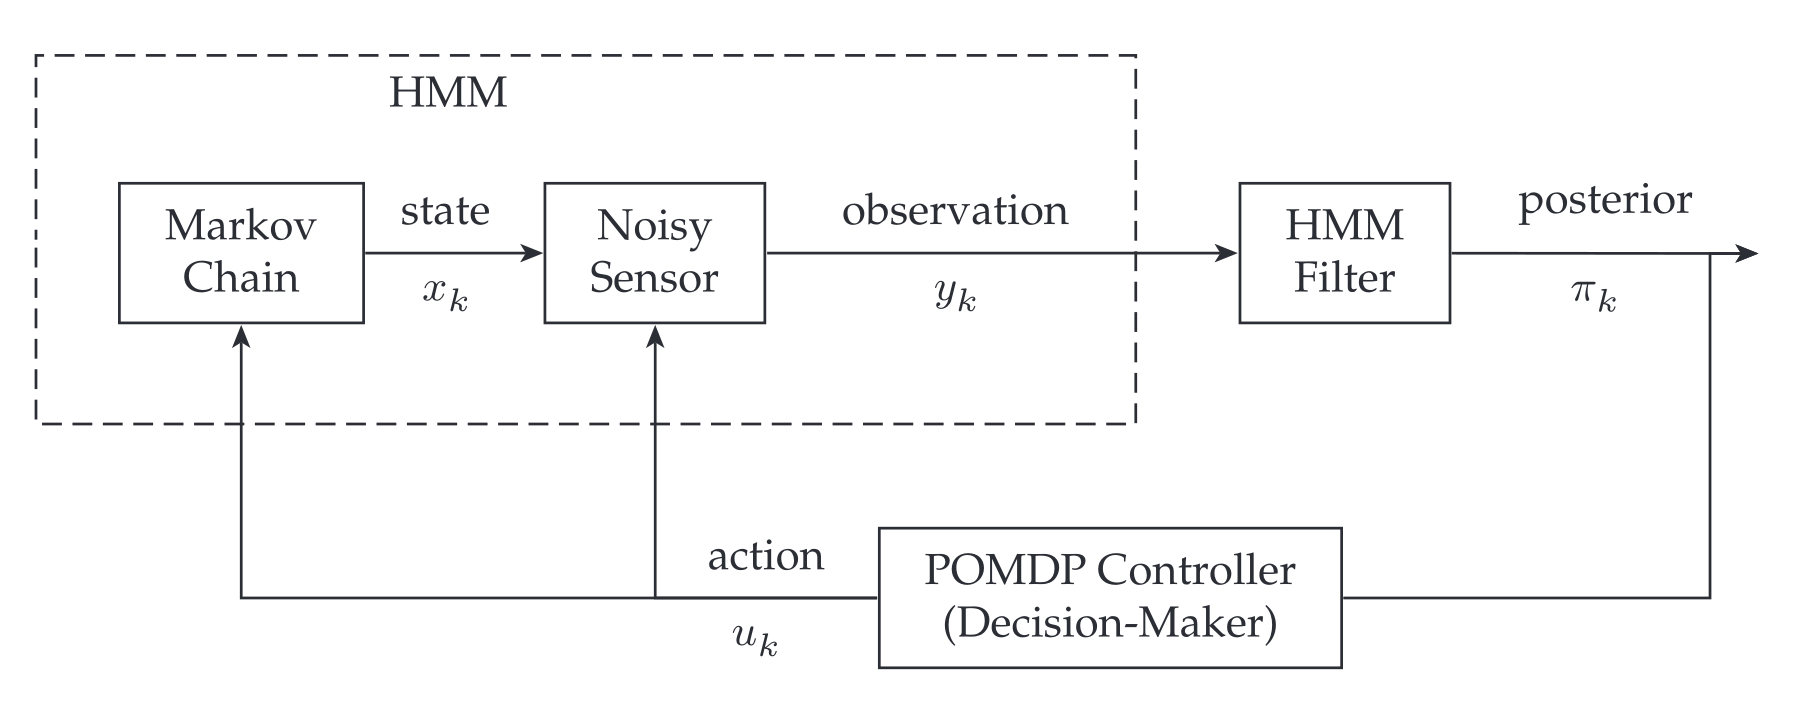
\includegraphics[scale=.15]{images/pomdp.png}
    \caption[Partially Observable Markov Decision Process]{Partially Observable Markov Decision Process \citep{Krishnamurthy_2016}}
    \label{fig:pomdp}
\end{figure}
As such \glspl{pomdp} are an extension of \glspl{mdp} to the case where the full observability assumption is 
relaxed in favour of a more general and realistic assumption that the agent only has partial knowledge 
of the state of the system but there exist observations/signals which yield probabilistic beliefs about 
the hidden state.

The next sections will be based on \cite{Spaan12pomdp} and \cite{Hauskrecht_2000} analysis of \glspl{pomdp},
originally introduced by the work of Drake, 1962; Astrom, 1965; Sondik, 1971;
Lovejoy, 1991b.
\todo{aggiusta citazioni }



\begin{definition}
A \textit{Partially Observable Markov Decision Process} is a tuple $P = (S, A,\Omega, \mathcal{T}, \mathcal{R}, \mathcal{O})$ where:
\begin{itemize}
    \setlength\itemsep{0.01em}
    \item $S$ is a finite set of states
    \item $A$ is a finite set of actions
    \item $\Omega$ is a finite set of observations
    \item $\mathcal{T}$ is the transition function $\mathcal{T} : S \times A \times S \rightarrow [0,1]$
    \item $\mathcal{R}$ is the reward function $\mathcal{R} : S \times A \times S \rightarrow \mathbb{R}$
    \item $\mathcal{O}$ is the observation function $\mathcal{O} : S \times A \times \Omega \rightarrow [0,1]$
\end{itemize}
\end{definition}


\begin{example}
    the need for memory (Singh et al, 1994).
\end{example}


In the next sections we will introduce the main concepts and algorithms used to solve \gls{pomdp}s.

\section{Belief State MDPs}
Since in \glspl{pomdp} the underliyng process states are unknown, the action choices will be based on the information available 
to the agent in the form of past actions and observations, giving rise to the concept of \textit{Information State}.

\begin{definition}
    (Complete Information State) the complete information state at time t denoted
    $I_t$ consists of:
    \begin{itemize}
        \item[-] prior belief $b_0$ on states in S at time $t=0$;
        \item[-] a complete history of actions and observations $\{o_0,a_0,o_1, ..., o_{t-1},a_{t-1},o_t\}$
    \end{itemize}
\end{definition}

A sequence of information states defines a controlled Markov process called 
information-state \gls{mdp}. In this context a policy $\pi: I \rightarrow A$ is mapping of 
information states to actions (possibly distributions over actions).
The new information state $I_{t+1}$ is obtained applying an update function $\tau$ to the
the previous state $I_t$, previous action $a_{t-1}$  and  observation $o_t$:
$$\tau: \mathcal{I} \times A \times O \rightarrow \mathcal{I}$$

It's easy to see that a \gls{pomdp} can be cast into the information-state MDP by using complete 
information states, revisiting the \gls{pomdp} such that states become information-states while transitions 
and rewards are updated accordingly
$$R(I,a) = \sum_{s s'} T(s,a,s')R(s,a,s')P(s|I) $$
$$T(I,a,I') = \sum_o \tau(I,a,o)P(o|I,a) $$


It's also important to note that the information available can be also summarized in the 
so called \textit{sufficient information states}. Such states must preserve
the necessary information content as well as the Markov property of the information-state.
\begin{definition}
    
    (Sufficient information state process). Let \(\mathcal{I}\) be an information state space 
    and \(\tau: \mathcal{I} \times A \times \Theta \rightarrow \mathcal{I}\) be an update function defining an information process \(I_{t}=\) 
    \(\tau\left(I_{t-1}, a_{t-1}, o_{t}\right)\). The process is sufficient with regard to the optimal control 
    if for every time step $t$, it satisfies
    $$P\left(s_{t} \mid I_{t}\right)=P\left(s_{t} \mid I_{t}^{C}\right)$$
    $$P\left(o_{t} \mid I_{t-1}, a_{t-1}\right)=P\left(o_{t} \mid I_{t-1}^{C}, a_{t-1}\right)$$
    where \(I_{t}^{C}\) and \(I_{t-1}^{C}\) are complete information states.

\end{definition} 
% \todo{definisci meglio p(s|I) e p(o|I,a)?? è necessario?}

Being able to define a sufficient information state process is crucial since it allows to avoid 
the curse of dimensionality of enlarging complete information states.

This brings us to the most common concept of \textit{belief state} as a form of sufficient information state
cite{strm1965OptimalCO}.

A belief is a probability distribution over the states of the system which summarizes the history of 
actions and observations. Each \gls{pomdp} assumes an initial belief $b_0$, then at each time step
the belief is updated by the observation and the action taken through Baye's rule.

$$\tau(b,a,o) = b^{ao}(s')=\displaystyle\frac{p(o|s',a)}{p(o|b,a)}\sum_{s\in S}p(s'|s,a)b(s)$$

where $p(s'|s,a) = T(s,a,s')$ and $p(o|s',a) = O(s,a,o)$, and
$$p(o|b,a)=\displaystyle\sum_{s'\in S}p(o|s',a)\sum_{s\in S}p(s'|s,a)b(s)$$.

It is thus possible to define a \gls{mdp} over belief states. 
This transformation requires the transition and observation functions to be known
to the agent, and hence can be applied only in model-based methods.

The key point is that belief-state \glspl{mdp} are fully
observable even though the original problem involves hidden quantities. This
formulation effectively turns the problem into a planning one in the space of beliefs.

Belief-state MDPs are the primary object of study in the field of \glspl{pomdp}

\section{Policies and Value Functions}
As in the fully observable context, the goal of the agent is to find a policy that maximizes the expected 
return. In the \gls{pomdp} case, the policy is a mapping from the set of probability distributions 
over $S$ as the value function $V^{\pi} : \Delta(S) \rightarrow \mathbb{R}$. 
In the infinite-horizon discounted case the value function is defined as:

$$V^{\pi}(b) \doteq \mathbb{E}_{\pi}\left[ \sum ^\infty _{t=0} \gamma^k R(b_t,\pi(b_t)) | b_0 = b  \right]$$

where $R(b_t,\pi(b_t)) = \sum_s R(s,\pi(b_t))b_t(s)$


Revisiting equations in previous section, the Bellman optimality equation for the value function 
in a belief space \gls{mdp} is given by:
$$V^* (b) = \max_a \left[\sum_s R(s,\pi(b_t))b_t(s) + \gamma\sum_o p(o|b,a) V^*(b'_{a,o}) \right]$$

or alternatively $V^* = HV^*$ where $H$ is the Bellman backup operator for \gls{pomdp}s defined as:
$$H V(b) = \max_a \left[\sum_s R(s,a)b(s) + \gamma\sum_o p(o|b,a) V(b'_{a,o}) \right]$$

The properties of the H operator are sufficient to guarantee the existence of a unique optimal value 
function given the Banach contraction theorem. \textit{Exact Value Iteration} is therefore formulated 
as the iterative application of the H operator to an initial value function until convergence - practically 
until the difference between the value function at two consecutive iterations is below a given threshold.
\todo{serve una dimostrazione H contrazione}
$$V_{n+1} = HV_n = H^n V_0$$ 


The major difficulty in applying exact value iteration is that the belief space is continuous and 
updates over the whole space are infeasible. 
Fortunately the value function can be parametrized by a finite set of vectors, the following result 
is originally from \cite{1307539f-051d-3d3c-a0d8-111443bed03f}.

\begin{theorem}
    (Piecewise linear and convex Value function). Let \(V_{0}\) be an initial value function
    that is piecewise linear and convex. Then the \(i\) th value function obtained after a finite
    number of update steps for a belief-state \gls{mdp} is also finite, piecewise linear and convex,
    and is equal to:
   
   \[
   V_{i}(b)=\max _{\alpha_{i} \in \Gamma_{i}} \sum_{s \in S} b(s) \alpha_{i}(s)
   \]
    where \(b\) and \(\alpha_{i}\) are vectors of size \(|S|\) and \(\Gamma_{i}\) is a finite set of vectors (linear functions) \(\alpha_{i}\).
\end{theorem}
\begin{proof}
It follows from induction. The result holds for the horizon one value function
$V_0 = \sum_s R(S,a)b(s)= \sum_{i}b_i\alpha_{0}^{i}(s)= b \cdot \alpha_0 $
Assuming the hypothesis holds for \(V_n\), we can show that it holds for \(V_{n+1}\) as well.
\begin{align*}
    V_{n+1}(b)&=\displaystyle\max_{a}\Big[\sum_s R(S,a)b(s)+\gamma\sum_{o}p(o|a,b)V_{n}(b_{a}^{o})\Big] \nonumber\\
    &=\displaystyle\max_{a}\Big[b\cdot r_{a}+\gamma\sum_{o}p(o|a,b)\max_{\{\alpha_{n}^{i}\}_{i}}\sum_{s^{\prime}}b_{a}^{o}(s^{\prime})\alpha_{n}^{i}(s^{\prime})\Big] \nonumber\\
    &=\displaystyle\max_{a}\Big[b\cdot r_{a}+\gamma\sum_{o}\max_{\{\alpha_{n}^{i}\}_{i}}\sum_{s^{\prime}}p(o|s^{\prime},a)\sum_{s}p(s^{\prime}|s,a)b(s)\alpha_{n}^{i}(s^{\prime})\Big] \nonumber\\
    &=\displaystyle\max_{a}\Big[b\cdot r_{a}+\gamma\sum_{o}\max_{\{g_{a,o}^{i}\}_{i}}b\cdot g_{a,o}^{i}\Big], \nonumber\\
    &=\displaystyle\max_{a}\Big[b\cdot r_{a}+\gamma b \cdot \sum_o arg\max_{\{g_{a,o}^{i}\}_{i}}b\cdot g_{a,o}^{i}\Big], \nonumber\\
    &=\displaystyle\max_{g_{a,o}}b \cdot g_a^b \nonumber
\end{align*}
denoting 
\[
\quad g_{a,o}^{i}(s)=\sum_{s^{\prime }}p(o|s^{\prime },a)p(s^{\prime
}|s,a)\alpha _{n}^{i}(s^{\prime }).\quad  
\]
and 
$$g_a^b = r_{a}+\gamma b \cdot \sum_o arg\max_{\{g_{a,o}^{i}\}_{i}}b\cdot g_{a,o}^{i} $$

therefore one can express the value function as stated.

\end{proof}

The main idea behind most value iteration algorithms is that for a given value function 
\(V_{n}\) and a single belief point \(b\) we can
easily compute the vector \(\alpha_{n+1}^{b}\) of \(H V_{n}\) such that
$$\alpha_{n+1}^{b}=\arg \max _{\left\{\alpha_{n+1}^{i}\right\}_{i}} b \cdot \alpha_{n+1}^{i}$$    
where \(\left\{\alpha_{n+1}^{i}\right\}_{i=1}^{|H V_{n}|}\) is the (unknown) set of vectors for \(H V_{n}\). 
We will denote this operation
\(\alpha_{n+1}^{b}=\operatorname{backup}(b)\). 
It computes the optimal vector for a given belief \(b\) by back-projecting
\begin{equation}
    {backup}(b)=\arg\max_{g_a^b} b\cdot g_a^b
    \label{eq:backup}
\end{equation}
        
% \todo{copiato da perseus dal teorema a qui}


Convexity of the value function the expected discounted reward generally grows as the entropy
of b decreases \Cref{fig:pomdp-value}.

\begin{figure}
    \centering
    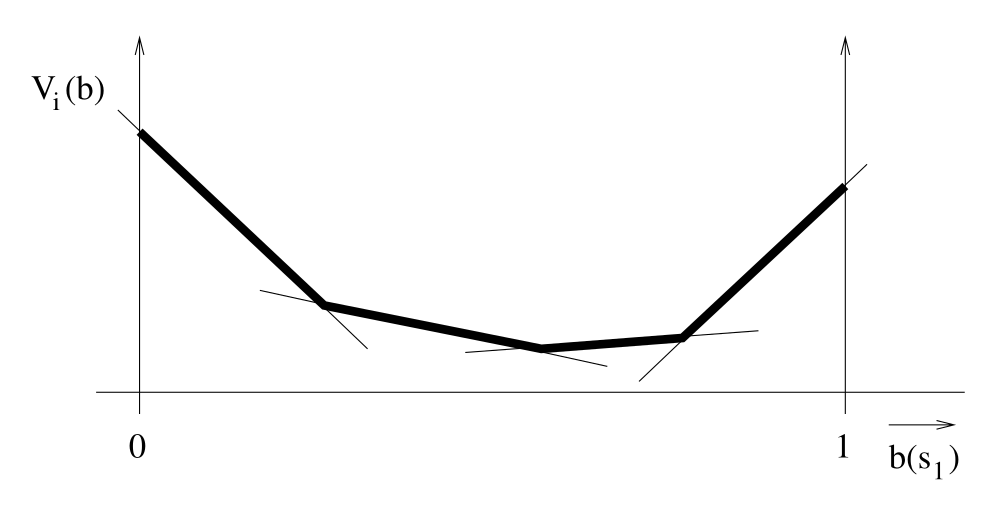
\includegraphics[scale=0.2]{images/pomdp-value.png}
    \caption{Convex Value function for a two states \gls{pomdp}.}
    \label{fig:pomdp-value}
\end{figure}

Even though the optimal value function for an infinite-horizon
\gls{pomdp} is convex, it may not be piecewise linear. Nontheless, it can be approximated
arbitrarily closely by a piecewise linear and convex value function.

The total number of all its possible linear functions is $|A|\Gamma_i|^{|O|}$ (one
for every combination of actions and permutations of $\alpha_i$ vectors of size $|O|$). 
% per trovare il massmo dentro le [] devo fissare azione e per ogni osservazione trovare l'alpha vector
% precedente associato che massimizza le somme su ss'

\paragraph{Policy}
Similarly to the \gls{mdp} case, in \glspl{pomdp} the optimal policy with respect to the Value function $V$ is:
$$\pi_{V}(b)=\underset{a}{\operatorname{argmax}} \left[R(b, a)+\gamma \sum_{o \in \Omega} \operatorname{Pr}\left(o \mid b, a\right) V\left(b^{a, o}\right)\right]$$
defined over the belief space.

Computing a policy for the current belief state \(b\) using the above equation requires computing
all the \(|A| \times|\Omega|\) successors of \(b\), with a cost of \(|S|^{2}\) for each successor. 
Then, computing the value at each successor requires \(|S| \times|V|\) operations 
(using the \(\alpha\)-vector representation).

However, we can label the vector resulting from the
point-based backup operation with the action associated with it. 
Then, all we need is to find the best $\alpha$-vector for the current
belief state and execute the corresponding action, with a computation cost of only $|S|\times|V |$ for 
finding the best action when following V.
\section{Exact Value Iteration}

The complete set of linear functions is rarely needed: some of the linear functions are 
dominated by others therefore not affecting the value function.
This approach - Sondik (1971) and Monahan (1982) - enumerates all possible linear functions
and then remove (prune) all redundant vectors. 
% Recent extensions of the
% method interleave the generate and test stages and do early pruning on a set of partially
% constructed linear functions (Zhang  Liu, 1997a; Cassandra, Littman,  Zhang, 1997;
% Zhang  Lee, 1998).

\todo{aggiusta O()}
This process is known as exact value iteration. In each iteration, the value function is
updated across the entire belief space. There are \(|V| \times|A| \times|\Omega|\) vectors generated at Eq. 21,
and computing each of these vectors takes \(|S|^{2}\) operations. In Eq. 19 we create \(|V|^{\Omega|}\) new
vectors for each action, with a complexity of \(|S|\) for each new vector. Hence, the overall
complexity of a single iteration is \(O\left(|V| \times|A| \times|\Omega| \times|S|^{2}+|A| \times|S| \times|V|^{\Omega|}\right)\).

\paragraph{Monahan’s Enumeration Algorithm}
\paragraph{Incremental Pruning}

An alternative approach builds on Sondik's idea of computing a useful linear function for a
single belief state (Sondik, 1971; Smallwood  Sondik, 1973), which can be done efficiently.
The key problem here is to locate all belief points that seed useful linear functions. 
Methods that implement this idea are Sondik's one- and two-pass algorithms (Sondik, 1971), 
Cheng's methods (Cheng, 1988), and the Witness algorithm 
(Kaelbling, Littman,  Cassandra, 1999; Littman, 1996; Cassandra,1998). 

\section{Point Based Value Iteration}
Approximate solution methods are necessary to solve \glspl{pomdp} in practice, since even modest 
sized problems are intractable with exact methods.
The main assumption behind \gls{pbvi} by \cite{10.5555/1630659.1630806} is that
it is unlikely to reach most of the points in the belief simplex.
Computing solutions only for those parts of the belief simplex that are reachable, i.e.,
that can be actually encountered by interacting with the environment, can drastically reduce 
the computational complexity of the problem.

the \gls{pbvi} algorithm solves a POMDP for a finite set of belief points $B$
initializing a $\alpha$-vector for each $b \in B$, and repeatedly updating 
(via value backups) the value of that $\alpha$-vector, preserving the piece-wise linearity 
and convexity of the value function, and defining value
function over the entire belief simplex.
\begin{figure}[H]
    \centering
    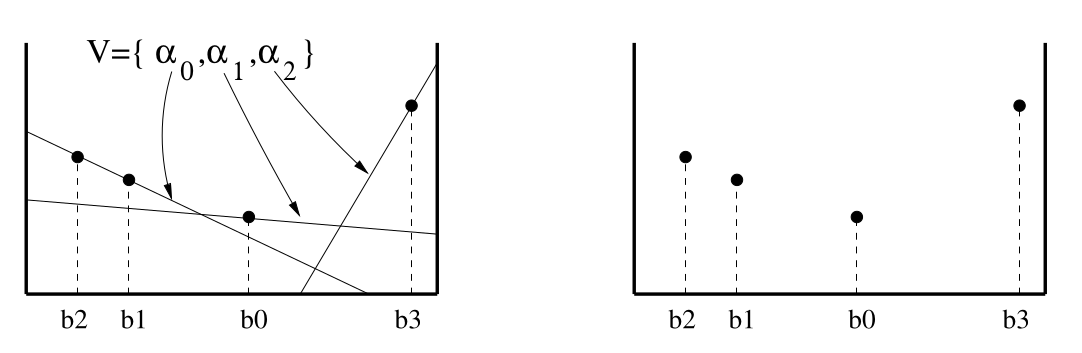
\includegraphics[scale=.35]{images/pbvi.png}
    \caption{Point-Based Value Iteration}
    \label{fig:pbvi}
\end{figure}



The point Based update follows exactly Eq. \ref{eq:backup} for each belief point in the set $B$. 
This is repeated h times for finite h-horizon problems, or a predefined number of iterations in the 
infinte case.

The next step is to enlarge the set of belief points by selecting for each belief \(b\) in \(B\) 
a successor \(b^{\prime}\) that is the most distant from the set \(B\). That is, let \(L\) be a 
distance metric, then define:
\[
\left|b^{\prime}-B\right|_{L}=\min _{b \in B}\left|b-b^{\prime}\right|_{L}
\]

and focus on candidate successors generated using forward simulation, thus:

\[
b^{\prime}=\max _{a, o}\left|b^{a, o}-B\right|_{L}
\] 

The set of successor points, one b for each b in Bi , are added into Bi (along with the previous
points in Bi ) to create the new set Bi+1 . Experiments by various researchers show little, if
any, sensitivity to the distance metric chosen, and L 1 has useful theoretical properties for the
convergence of PBVI. The full procedure is formally described in Algorithm


The complexity of computing $g_{a,o}^{i}$ is \(O\left(|S|^{2}\right)\), and it is done for every \(\alpha \in V\), hence
 computing all $g^{a, o}$ requires \(O\left(|A| \times|\Omega| \times|V| \times|S|^{2}\right)\). Computing \(\alpha_{a}^{b}\) (Eq. 34) requires the
 computation of all the relevant \(\alpha^{a, o}\), but then the summation and inner products require only
 \(O(|S| \times|\Omega|)\) operations and another \(O(|S|)\) operations for adding the reward vector. Finally,
 the backup operation requires for each \(\alpha_{a}^{b}\) another \(O(|S|)\) operations for the inner
 product. Hence, the full complexity of the point-based backup requires \(O(|A| \times|\Omega| \times|V| \times\)
 \(|S|^{2}+|A| \times|S| \times|\Omega|\) ).



However, a full backup for the subset \(B\) will not require \(|B|\) times the complexity of a
 single point-based backup, because the \(\alpha^{a, o}\) are independent of the current belief point \(b\).
 Hence, executing a backup for \(|B|\) belief points over a single value function \(V\), where we
 compute every \(\alpha^{a, o}\) only once and cache the result, requires only \(O(|A| \times|\Omega| \times|V| \times|S|^{2}+\)
 \(|B| \times|A| \times|S| \times|\Omega|\) ), as compared with the \(O(|A| \times|\Omega| \times|V| \times|S|^{2}+|A| \times|S| \times|V|^{\Omega|})\)
 of a single iteration of the exact backup. 

 \paragraph{Proof of convergence bounds} \cite{10.5555/1630659.1630806}
\subsection{Perseus}

\cite{Spaan_2005}
This scheme is a heuristic to let Bt cover a wide area of the belief space,
but comes at a cost as it requires computing distances between all b Bt . By backing up
all b Bt the PBVI algorithm generates at each stage approximately  vectors, which
can lead to slow performance in domains requiring large Bt .
In the next section we will present a point-based POMDP value iteration method which
does not require backing up all b  B. We compute backups for a subset of B only, but
seeing to it that the computed solution will be effective for the complete set B. As a result
we limit the growth of the number of vectors in the successive value function estimates,
leading to significant speedups.

% As each b has a region in the belief space in which its
% nb is maximal, a family of algorithms tries to identify these regions (Sondik, 1971;
% Cheng, 1988; Kaelbling et al, 1998). The corresponding b of each region is called
% a “witness” point, as it testifies to the existence of its region. Other exact POMDP
% value-iteration algorithms do not focus on searching in the belief space. Instead, they
% consider enumerating all possible vectors of HPOMDPVn , followed by pruning useless
% vectors (Monahan, 1982; Zhang and Liu, 1996; Littman, 1996; Cassandra et al,
% 1997; Feng and Zilberstein, 2004; Lin et al, 2004; Varakantham et al, 2005). We will
% focus on the enumeration algorithms as they have seen more recent developments
% and are more commonly used..

\section{Heuristics Approximations}
\subsection{QMDP}
\subsection{action voting}
\subsection{most likely state}
\subsection{entropy heuristics}
Cassandra [1998] shows how to use the entropy
of b to switch between information gathering policies and exploitive policies.
The entropy can also be used to weight two policies that trade off information
gathering and exploitation. These heuristics may be misleading if the minimum
of (b) does not occur at the point of greatest entropy, that is, the uniform
belief state.

\section{Model Free et al}
5. Function Approximation Methods

These methods use machine learning techniques to approximate value functions or policies.

    Deep Reinforcement Learning (DRL) for POMDPs: Uses neural networks to approximate value functions or policies.
    Deep Q-Networks (DQN) with Recurrent Layers: Uses LSTMs to track hidden states in partially observable environments.

% Model-based approaches tend to be more complex
% computationally than model-free ones, but they allow for prior knowledge of the
% environment to be more naturally incorporated in the learning process.

\part{Experiments}

\chapter{Methods}
We adopted a bottom up approach, increasing the complexity of the task in increasingly complex environments.
Recall that our objective was to explore the applicability of \gls{rl} to navigation in 
deformable environment related to the surgical task of thoracic surgery.
We therefore adopted a mixed approach assuming the model of the environment to be known or learnable, 
given the preoperative imaging data available in the clinical setting. This would allow us to model 
the problem as a \gls{pomdp} and apply the methods described in the previous sections.

\section{Gridworld}
The first task we considered was a simple gridworld, where the agent had to navigate from a random 
starting position to a goal position. The twist is given by the deformable property of the environment.

\paragraph{State Space}

The state space is a 2D grid of size $10 \times 10$ where each cell can be either empty or occupied by an obstacle.
the state is represented as a tuple $(x,y,\phi)$ where $x$ and $y$ are the coordinates of the agent in the grid.
and $\phi$ is the orientation of the agent.

\paragraph{Action Space}

The agent can move in four directions: up, down, left, right. The action space is therefore $A = \{0,1,2,3\}$.

\paragraph{Observation Space}

Every time the agent moves, it receives an observation which corresponds to the type of adjacent cells 
in the grid.  


The **conditional observation probabilities** $O(o|s,a)$ are also deterministic.


$$O(o|s,a)= O(o|s) = 
\begin{cases}
    1 &   \text{if } (x,y) \text{ adjacent cells for map } f_\theta(M) \text{are compatible with } o \\
    0 &   \text{otherwise} \\
\end{cases}
$$

\paragraph{Reward Function}


The **reward function** $R(s,a,s')$ is defined as follows:


 $$R(s,a,s') = 
    \begin{cases}
    \frac{-0.1}{mapsize} &   s' \neq s_{goal} \wedge \text{moved} \\ 
    \frac{-0.2}{mapsize} &   s' \neq s_{goal}  \wedge \text{hit wall}\\
    1 &   s' = s_{goal} \\
    \end{cases}    
$$

\paragraph{Transition Function}
Always assuming deterministic transitions, the transition function is defined as follows:
$$T(s'|s,a) =
\begin{cases}
    1 &   \text{if } s' \text{ is the result of applying action } a \text{ to state } s \\
    0 &   \text{otherwise} \\
\end{cases}
$$

\paragraph{Observation Function}

\paragraph{Belief State}
Because the agent does not directly observe the environment's state, the agent must make decisions under uncertainty of the true environment state. The belief function is a probability distribution over the states of the environment.

$$b : S \rightarrow [0,1] \text{ and } \sum_s b(s) = 1  $$

By interacting with the environment and receiving observations, the agent may update its belief in the true state by updating the probability distribution of the current state

$$ b'(s')=\eta O(o\mid s',a)\sum _{s\in S}T(s'\mid s,a)b(s)$$

where $\eta = \frac{1}{Pr ( o | b , a )}$ is a normalizing constant with 
$$Pr ( o | b , a ) = \sum_{s'\in S} O ( o | s' , a ) \sum_{s \in S}( s'|s,a)b(s)$$

Discrete update of the belief state is done by the agent at each time step.


\section{Deformable Maze}

\paragraph{State Space}
\paragraph{Action Space}
\paragraph{Observation Space}
\paragraph{Reward Function}
\paragraph{Transition Function}
\paragraph{Observation Function}
\section{Surgical Task}

\paragraph{State Space}
\paragraph{Action Space}
\paragraph{Observation Space}
\paragraph{Reward Function}
\paragraph{Transition Function}
\paragraph{Observation Function}
\chapter{Results}
Presentation of results...
GraspLiftAndTouchEnv models a sub-task from laparoscopic chole-
cystectomy, i.e., the minimally invasive removal of the gallbladder. Dur-
ing dissection of the yellow gallbladder from the red liver, the blue
grasper has to grasp the distal end (infundibulum) of the partially re-
sected gallbladder. Afterwards, the grasper retracts the gallbladder,
exposing a visual marker, which represents the point that should be
cut next. The green electrocautery hook then navigates to the visual
marker and activates in order to cut the tissue. The task is complete
when the target is visible to the camera and the cauter activates while
touching it.

\chapter{Future Directions}

Simulation-based pretraining to reduce real-world data collection costs.
Transfer learning from simpler robotic tasks (e.g., grasping) to more complex surgical tasks.
Safety-aware RL methods (constrained policies) to minimize surgical risk.
Domain adaptation techniques to handle variations in patient anatomy and real-time changes.
Hybrid approaches that blend model-based and model-free RL for adaptive decision-making and uncertainty handling.

% Bibliography
% \printbibliography
\bibliographystyle{plainnat}  % or abbrvnat, unsrtnat, etc.
\bibliography{ref}  % Name of your .bib file (without extension)
% \bibliographystyle{plain}
% \bibliography{ref}

% Appendix (optional)
\appendix
\chapter{Appendix A}
\section{Operators and Contractions}

% again putterman 1994
% There are (at least) two versions of policy evaluation: a synchronous one and an asynchronous one. 

% In the **synchronous** version (SPE), you maintain two arrays for the values of the states: one array holds the current values of the states and the other array will contain the next values of the states, so two arrays are used in order to be able to update the value of each state at the same time. 

% In the **asynchronous** version (APE), you update the value of each state in place. So, first, you update the value of e.g. $s_1$, then $s_2$, etc., by changing your only array of values (so you do not require a second array).

% SPE is similar in style to the numerical method called [Jacobi method][3], which is a general iterative method for finding a solution to a system of linear equations (which is exactly what PE is actually doing, and this is also explained in the cited book by Sutton and Barto). Similarly, APE is similar in style to [the Gauss–Seidel method][4], which is another method to solve a system of linear equations.

% Both of these general numerical methods to solve a system of linear equations are studied in detail in [Parallel and Distributed Computation Numerical Methods][2] (1989) by Bertsekas and Tsitsiklis, which I haven't read yet, but provides convergence results for these numerical methods.

% The book [Reinforcement learning: an introduction][1] by Sutton and Barto provides a more detailed description of policy evaluation (PE). 

%  Proof of convergence

% I will provide a proof for the SPE based on [these slides][5] by [Tom Mitchell][6]. Before proceeding, I suggest you read the following question  [What is the Bellman operator in reinforcement learning?][7] and its answer, and you should also get familiar with vector spaces, norms, fixed points and maybe contraction mappings.

% The proof that PE finds a unique fixed-point is based on the **contraction mapping theorem** and on the concept of **$\gamma$-contractions**, so let me first recall these definitions.

% > **Definition ($\gamma$-contraction)**: An operator on a normed vector space $\mathcal{X}$ is a $\gamma$-contraction, for $0 < \gamma < 1$, provided for all  $x, y \in \mathcal{X}$
% >
% > $$\| F(x) - F(y) \| \leq \gamma \| x - y\|$$
% >
% > **Contraction mapping theorem**: For a $\gamma$-contraction $F$ in a complete normed vector space $\mathcal{X}$
% >
% > - Iterative application of $F$ converges to a **unique** fixed point in $\mathcal{X}$ independently of the starting point
% >
% > - at a linear convergence rate determined by $\gamma$

% Now, consider the vector space $\mathcal{V}$ over state-value functions $v$ (i.e. $v \in \mathcal{V})$. So, each point in this space fully specifies a value function $v : \mathcal{S} \rightarrow \mathbb{R}$ (where $\mathcal{S}$ is the state space of the MDP).

% **Theorem (convergence of PE)**: The [Bellman operator][7] is a $\gamma$-contraction operator, so an iterative application of it converges to a unique fixed-point in $\mathcal{V}$. Given that PE is an iterative application of the Bellman operator (see [What is the Bellman operator in reinforcement learning?][7]), PE finds this unique fixed-point solution.

% So, we just need to show that the Bellman operator is a $\gamma$-contraction operator in order to show that PE finds this unique fixed-point solution.

%  Proof

% We will measure the distance between state-value functions $u$ and $v$ by the $\infty$-norm, i.e. the largest difference between state values:

% $$\|u - v\|_{\infty} = \operatorname{max}_{s \in \mathcal{S}} |u(s) - v(s)|$$

% **Definition (Bellman operator)**: We define the Bellman expectation operator as

% $$F^\pi(v) = \mathbf{r}^\pi + \gamma \mathbf{T}^\pi v$$

% where $v \in \mathcal{V}$, $\mathbf{r}^\pi$ is an $|\mathcal{S}|$-dimensional vector whose $j$th entry gives $\mathbb{E} \left[ r \mid s_j, a=\pi(s_j) \right]$ and $\mathbf{T}^\pi$ is an $|\mathcal{S}| \times |\mathcal{S}|$ matrix whose $(j, k)$ entry gives $\mathbb{P}(s_k \mid s_j, a=\pi(s_j))$.

% Now, let's measure the distance (with the $\infty$-norm defined above) between any two value functions $u \in \mathcal{V}$ and $v \in \mathcal{V}$ after the application of the Bellman operator $F^\pi$ 

% \begin{align}
% \| F^\pi(u) - F^\pi(v) \|_{\infty} 
% &= \| (\mathbf{r}^\pi + \gamma \mathbf{T}^\pi u) - (\mathbf{r}^\pi + \gamma \mathbf{T}^\pi v)\|_{\infty} \\
% &= \| \gamma \mathbf{T}^\pi (u - v)\|_{\infty} \\
% &\leq \| \gamma \mathbf{T}^\pi ( \mathbb{1} \cdot \| u - v \|_{\infty})\|_{\infty} \\
% &\leq \| \gamma (\mathbf{T}^\pi \mathbb{1}) \cdot \| u - v \|_{\infty}\|_{\infty} \\
% &\leq \gamma \| u - v \|_{\infty}
% \end{align}

% where $\mathbb{1} = [1, \dots, 1]^T$. Note that $\mathbf{T}^\pi \cdot \mathbb{1} = \mathbb{1}$ because $\mathbf{T}^\pi$ is a [stochastic matrix][8].

% By the Bellman expectation equation (see Barto and Sutton's book and [What is the Bellman operator in reinforcement learning?][7]), $v^\pi$ is **a** fixed-point of the Bellman operator $F^\pi$. Given the contraction mapping theorem, the iterative application of $F^\pi$ produces a **unique** solution, so $v^\pi$ must be this unique solution, i.e. SPE finds $v^\pi$. [Here][12] is another version of the proof that the Bellman operator is a contraction.


\end{document}



% \begin{algorithm}[H]
%     \begin{algorithmic}
%     \Procedure{PolicyIteration}{$\mathcal{X}$, $A$, $g$, $f$, $F$, $\alpha$}
%         \State Initialize $\pi$ arbitrarily
%         \While{$\pi$ is not converged}
%             \State $J \gets$ solve system of linear equations $(I - \alpha \cdot F(\pi)) \cdot J = g(\pi)$

%             \For{$x \in \mathcal{X}$}
%                 \For{$a \in A(x)$}
%                     \State $Q(x, a) \gets g(x, a) + \alpha \sum_{j=1}^{n_x} f_{xj}(a) \cdot J(j)$
%                 \EndFor
%             \EndFor
%             \For{$x \in \mathcal{X}$}
%                 \State $\pi(x) \gets \arg \min_a \{Q(x, a)\}$
%             \EndFor
%         \EndWhile
%         \Return $\pi$
%     \EndProcedure
%     \end{algorithmic}
% \caption{Policy Iteration: Learning a policy $\pi: \mathcal{X} \rightarrow \mathcal{A}$}
% \label{alg:policy-iteration}
% \end{algorithm}


% \begin{algorithm}[H]
%     \begin{algorithmic}
%     \Require
%     \Statex Sates $\mathcal{X} = \{1, \dots, n_x\}$
%     \Statex Actions $\mathcal{A} = \{1, \dots, n_a\},\qquad A: \mathcal{X} \Rightarrow \mathcal{A}$
%     \Statex Cost function $g: \mathcal{X} \times \mathcal{A} \rightarrow \mathbb{R}$
%     \Statex Transition probabilities $f_{xy}(a) = \mathbb{P}(y | x, a)$
%     \Statex Discounting factor $\alpha \in (0, 1)$, typically $\alpha = 0.9$
%     \Procedure{ValueIteration}{$\mathcal{X}$, $A$, $g$, $f$, $\alpha$}
%         \State Initialize $J, J': \mathcal{X} \rightarrow \mathbb{R}_0^+$ arbitrarily
%         \While{$J$ is not converged}
%             \State $J' \gets J$
%             \For{$x \in \mathcal{X}$}
%                 \For{$a \in A(x)$}
%                     \State $Q(x, a) \gets g(x, a) + \alpha \sum_{j=1}^{n_x} f_{xj}(a) \cdot J'(j)$
%                 \EndFor
%             \EndFor
%             \For{$x \in \mathcal{X}$}
%                 \State $J(x) \gets \min_a \{Q(x, a)\}$
%             \EndFor
%         \EndWhile
%         \Return $J$
%     \EndProcedure
%     \end{algorithmic}
% \caption{Value Iteration: Learn function $J: \mathcal{X} \rightarrow \mathbb{R}$}
% \label{alg:value-iteration}
% \end{algorithm}